%%%%%%%%%%%%%%%%%%%%%%%%%%%%%%%%%%%%%%%%%%%%%%%%%%%
\begin{frame}
  \begin{center}
    {\Large Neural Networks can compute ANY function!!!}
    
    {\tiny (Ref: A visual proof that neural nets can compute any function - Michael Nielsen, Dec 2017)}
  \end{center}
\end{frame}

% %%%%%%%%%%%%%%%%%%%%%%%%%%%%%%%%%%%%%%%%%%%%%%%%%%%%%%%%%%%%%%%%%%%%%%%%%%%%%%%%%%
% \begin{frame}[fragile]\frametitle{Core Idea}

% What's the core idea  \ldots
% \begin{itemize}
% \item behind problem solving?
% \item behind writing software algorithms?
% \item solving research problems?
% \item all of the above, either using traditional ways, or ML-DL ways \ldots
% \end{itemize}
% \end{frame}

% %%%%%%%%%%%%%%%%%%%%%%%%%%%%%%%%%%%%%%%%%%%%%%%%%%%%%%%%%%%
% \begin{frame}[fragile]\frametitle{Desire}
% \begin{itemize}
% \item To find a ``function''
% \item To find a relation
% \item To find a transformation
% \item To build a model
% \item From given inputs to desired outputs.
% \end{itemize}
% That's it.
% \end{frame}

% %%%%%%%%%%%%%%%%%%%%%%%%%%%%%%%%%%%%%%%%%%%%%%%%%%%%%%%%%%%
% \begin{frame}[fragile]\frametitle{Functions}
% \begin{itemize}
% \item Some functions are straight forward
% \item {\em ``In summer, ice-cream sale goes up''}
% \item Cause and effect
% \item Relation (function, Mathematical model) is found out
% \item Here, simple rule based programming suffices
% \end{itemize}
% \end{frame}

% %%%%%%%%%%%%%%%%%%%%%%%%%%%%%%%%%%%%%%%%%%%%%%%%%%%%%%%%%%%
% \begin{frame}[fragile]\frametitle{Functions}
% \begin{itemize}
% \item But some functions are complex
% \item {\em ``More you put efforts, your business flourishes.''}
% \item Cause and effect again, but the relation is far to complex
% \item Too many variables
% \item Here, simple rule based programming not humanly possible.
% \item Lots of research needed to come up with equations.
% \end{itemize}

% \end{frame}

%%%%%%%%%%%%%%%%%%%%%%%%%%%%%%%%%%%%%%%%%%%%%%%%%%%%%%%%%%%
\begin{frame}[fragile]\frametitle{Functions}
\begin{itemize}
\item Can there be a way: given inputs and outputs, SOMEONE gives us the function?
\item Well, there is.
\item May be approximately (in a practical settings).
\end{itemize}


\end{frame}

%%%%%%%%%%%%%%%%%%%%%%%%%%%%%%%%%%%%%%%%%%%%%%%%%%%
\begin{frame}[fragile] \frametitle{A Striking Fact}
\begin{itemize}
\item Neural Networks can compute ANY function.
\item Even a complicated function like $f(x)$:
\end{itemize}

\begin{center}
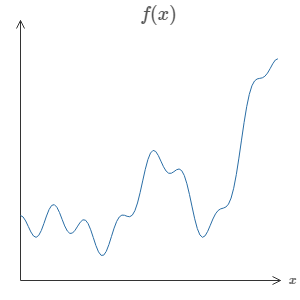
\includegraphics[width=0.5\linewidth,keepaspectratio]{dmaths1}
\end{center}
\end{frame}

%%%%%%%%%%%%%%%%%%%%%%%%%%%%%%%%%%%%%%%%%%%%%%%%%%%
\begin{frame}[fragile] \frametitle{A Striking Fact}
No matter what the function, there is guaranteed to be a neural network so that for every possible input, $x$, the value $f(x)$ (or some close approximation) is output from the network, e.g.

\begin{center}
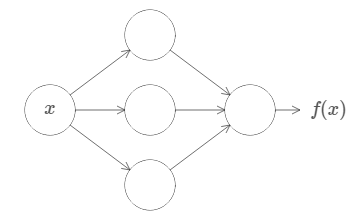
\includegraphics[width=0.7\linewidth,keepaspectratio]{dmaths2}
\end{center}
\end{frame}

%%%%%%%%%%%%%%%%%%%%%%%%%%%%%%%%%%%%%%%%%%%%%%%%%%%
\begin{frame}[fragile] \frametitle{A Striking Fact}
Possible even when the function has many inputs, $f=f(x_1,\ldots,x_m)$, and many outputs. For instance, here's a network computing a function with $m=3$ inputs and $n=2$ outputs:

\begin{center}
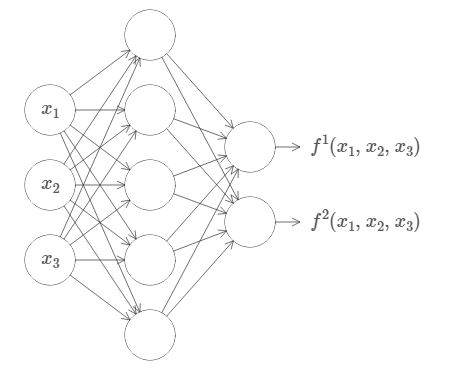
\includegraphics[width=0.4\linewidth,keepaspectratio]{dmaths3}
\end{center}

Meaning, neural networks have a kind of universality. No matter what function we want to compute, we know that there is a neural network which can do the job.
\end{frame}



%%%%%%%%%%%%%%%%%%%%%%%%%%%%%%%%%%%%%%%%%%%%%%%%%%%
\begin{frame}[fragile] \frametitle{Universality Theorem}
\begin{center}
{\Large Any continuous function $f$ can be realized by a network with one hidden layer, given enough hidden neurons.}
\end{center}

\end{frame}


%%%%%%%%%%%%%%%%%%%%%%%%%%%%%%%%%%%%%%%%%%%%%%%%%%%%
%\begin{frame}[fragile] \frametitle{Universality Theorem}
%THEN, why ``Deep'' neural network not ``Fat'' neural network? (will see later)
%\begin{center}
%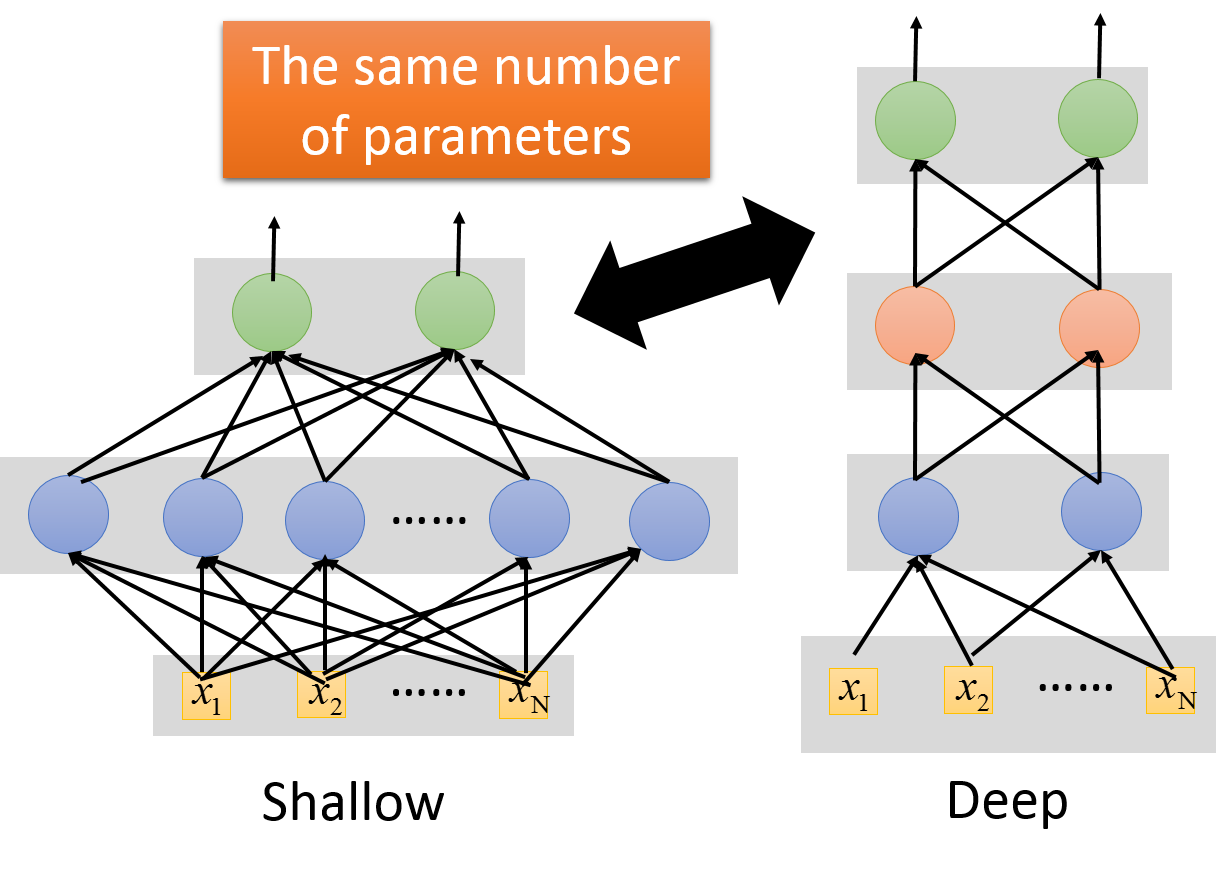
\includegraphics[width=0.8\linewidth,keepaspectratio]{fatdeep}
%\end{center}
%\end{frame}

%%%%%%%%%%%%%%%%%%%%%%%%%%%%%%%%%%%%%%%%%%%%%%%%%%%
\begin{frame}[fragile] \frametitle{Compute ANY function?}
\begin{itemize}
\item Well, at least approximately for sure, depending on the architecture.
\begin{center}
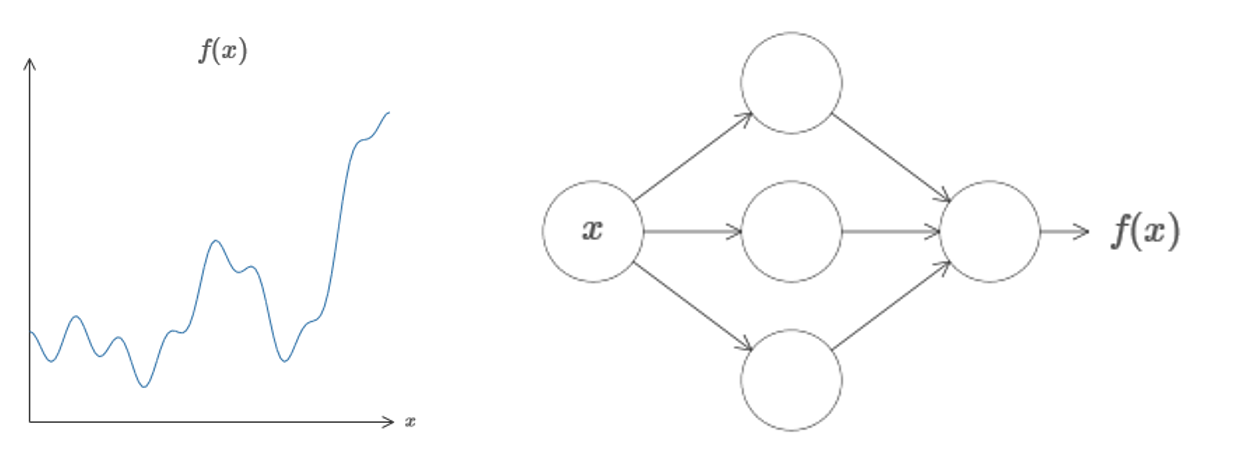
\includegraphics[width=\linewidth,keepaspectratio]{anyfunc}
\end{center}
\item For every value of $x$ there will be correct (approximate) value of $f(x)$
\end{itemize}

{\tiny (Ref: http://neuralnetworksanddeeplearning.com/chap4.html)}

\end{frame}

%%%%%%%%%%%%%%%%%%%%%%%%%%%%%%%%%%%%%%%%%%%%%%%%%%%
\begin{frame}[fragile] \frametitle{More advanced: Many inputs, Many Outputs}
\begin{itemize}
\item A function with multiple inputs, $f = f(x_1,x_2,,,x_m)$
\item A set of different functions with different inputs
\end{itemize}
\begin{center}
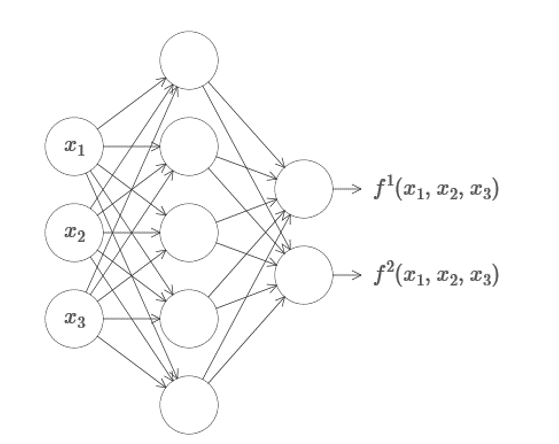
\includegraphics[width=0.5\linewidth,keepaspectratio]{moreadv}
\end{center}

{\tiny (Ref: http://neuralnetworksanddeeplearning.com/chap4.html)}
\end{frame}

%%%%%%%%%%%%%%%%%%%%%%%%%%%%%%%%%%%%%%%%%%%%%%%%%%%
\begin{frame}[fragile] \frametitle{Universality: Two caveats}
First caveat: Approximation
\begin{itemize}
\item This Universality doesn't mean that a network can be used to exactly compute any function.
\item Rather, we can get an approximation that is as good as we want. 
\item By increasing the number of hidden neurons we can improve the approximation.
\item With 3 neurons we get low quality approximation, with 5, better than that, and so on.
\end{itemize}
\begin{center}
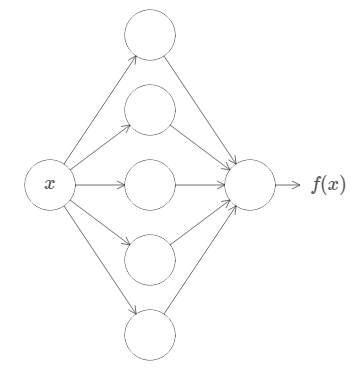
\includegraphics[width=0.2\linewidth,keepaspectratio]{dmaths4}
\end{center}
{\tiny (Ref: http://neuralnetworksanddeeplearning.com/chap4.html)}
\end{frame}

%%%%%%%%%%%%%%%%%%%%%%%%%%%%%%%%%%%%%%%%%%%%%%%%%%%
\begin{frame}[fragile] \frametitle{Universality: Two caveats}
Approximation, mathematically speaking \ldots
\begin{itemize}
\item Suppose we're given a function $f(x)$ which we'd like to compute to within some desired accuracy $\epsilon >0$. 
\item The guarantee is that by using enough hidden neurons we can always find a neural network whose output $g(x)$ satisfies $|g(x)- f(x)|<\epsilon$, for all inputs $x$. 
\item In other words, the approximation will be good to within the desired accuracy for every possible input.
\end{itemize}

{\tiny (Ref: http://neuralnetworksanddeeplearning.com/chap4.html)}
\end{frame}

%%%%%%%%%%%%%%%%%%%%%%%%%%%%%%%%%%%%%%%%%%%%%%%%%%%
\begin{frame}[fragile] \frametitle{Universality: Two caveats}
Second caveat: Continuous functions
\begin{itemize}
\item Function that needs to be approximated should be continuous.
\item If a function is discrete or discontinuous, i.e., makes sudden, sharp jumps, gaps, etc then it won't in general be possible to approximate using a neural net.
\end{itemize}

{\tiny (Ref: http://neuralnetworksanddeeplearning.com/chap4.html)}
\end{frame}

%%%%%%%%%%%%%%%%%%%%%%%%%%%%%%%%%%%%%%%%%%%%%%%%%%%
\begin{frame}[fragile] \frametitle{Universality: One input One Output}
Let's start with a network containing just a single hidden layer, with two hidden neurons, and an output layer containing a single output neuron:
\begin{center}
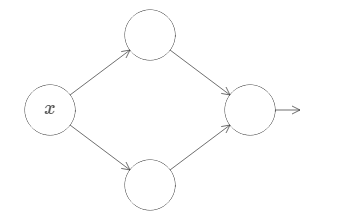
\includegraphics[width=0.5\linewidth,keepaspectratio]{dmaths5}
\end{center}

\begin{itemize}
\item Input is $x$, and there is only one output $f(x)$. 
\item Each arrow has weight $w$. 
\item Each node is associated with a bias $b$
\item At the top hidden node the input is transformed into $wx+b$
\end{itemize}

{\tiny (Ref: http://neuralnetworksanddeeplearning.com/chap4.html)}
\end{frame}

%%%%%%%%%%%%%%%%%%%%%%%%%%%%%%%%%%%%%%%%%%%%%%%%%%%
\begin{frame}[fragile] \frametitle{Universality: One input One Output}
\begin{itemize}
\item On top of the wighted sum + bias, an activation function like sigmoid is applied to introduce non-linearity. 
\item So eqn becomes $\sigma(wx+b)$, where $\sigma(z) = 1/(1+e^{-z})$
\item We can see effect of change in $w$ and $b$ on the shape of the output.
\end{itemize}

\begin{center}
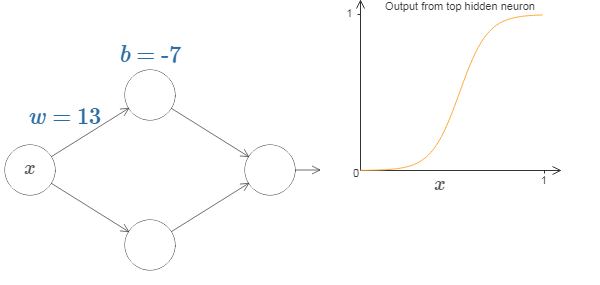
\includegraphics[width=0.7\linewidth,keepaspectratio]{dmaths6}
\end{center}


{\tiny (Ref: http://neuralnetworksanddeeplearning.com/chap4.html)}
\end{frame}

%%%%%%%%%%%%%%%%%%%%%%%%%%%%%%%%%%%%%%%%%%%%%%%%%%%
\begin{frame}[fragile] \frametitle{Universality: One input One Output}
Change in $w$

\begin{center}
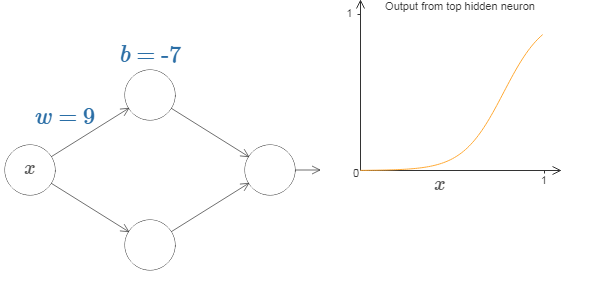
\includegraphics[width=0.6\linewidth,keepaspectratio]{dmaths7}
\end{center}

\begin{center}
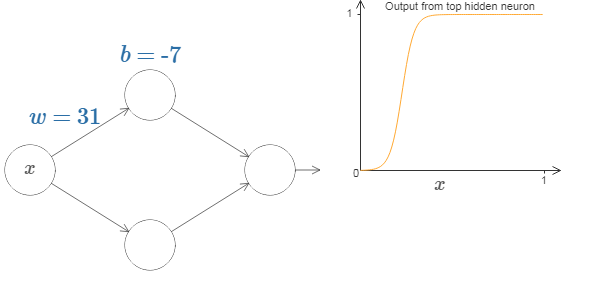
\includegraphics[width=0.6\linewidth,keepaspectratio]{dmaths8}
\end{center}

{\tiny (Ref: http://neuralnetworksanddeeplearning.com/chap4.html)}
\end{frame}

%%%%%%%%%%%%%%%%%%%%%%%%%%%%%%%%%%%%%%%%%%%%%%%%%%%
\begin{frame}[fragile] \frametitle{Universality: One input One Output}
Change in $b$

\begin{center}
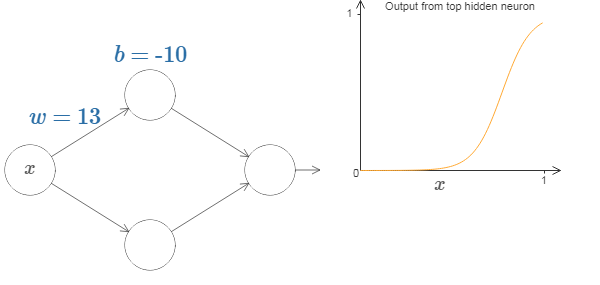
\includegraphics[width=0.6\linewidth,keepaspectratio]{dmaths9}
\end{center}

\begin{center}
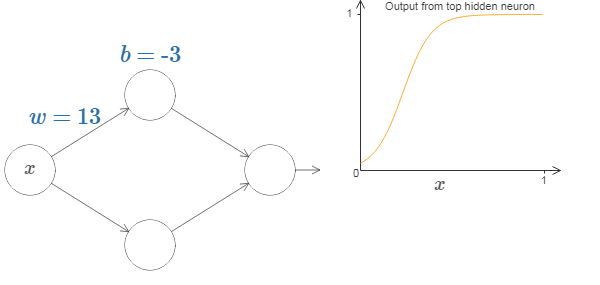
\includegraphics[width=0.6\linewidth,keepaspectratio]{dmaths10}
\end{center}

{\tiny (Ref: http://neuralnetworksanddeeplearning.com/chap4.html)}
\end{frame}


%%%%%%%%%%%%%%%%%%%%%%%%%%%%%%%%%%%%%%%%%%%%%%%%%%%
\begin{frame}[fragile] \frametitle{Universality: One input One Output}
\begin{itemize}
\item As the bias decreases the graph moves to the right, but, again, its shape doesn't change.
\item As you decrease the weight, the curve broadens out. 
\item Finally, increase the weight up past $w=100$. As you do, the curve gets steeper, until eventually it begins to look like a step function. 
\item Adjust the bias so the step occurs near $x=0.3$
\end{itemize}

\begin{center}
%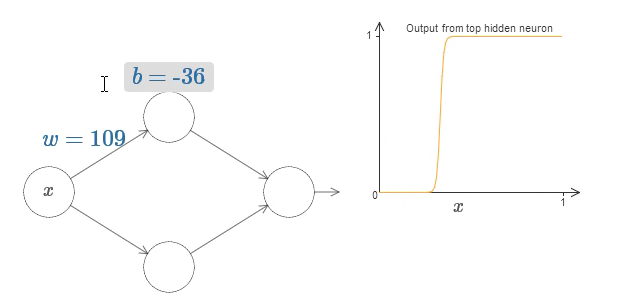
\includegraphics[width=0.6\linewidth,keepaspectratio]{dmaths11}
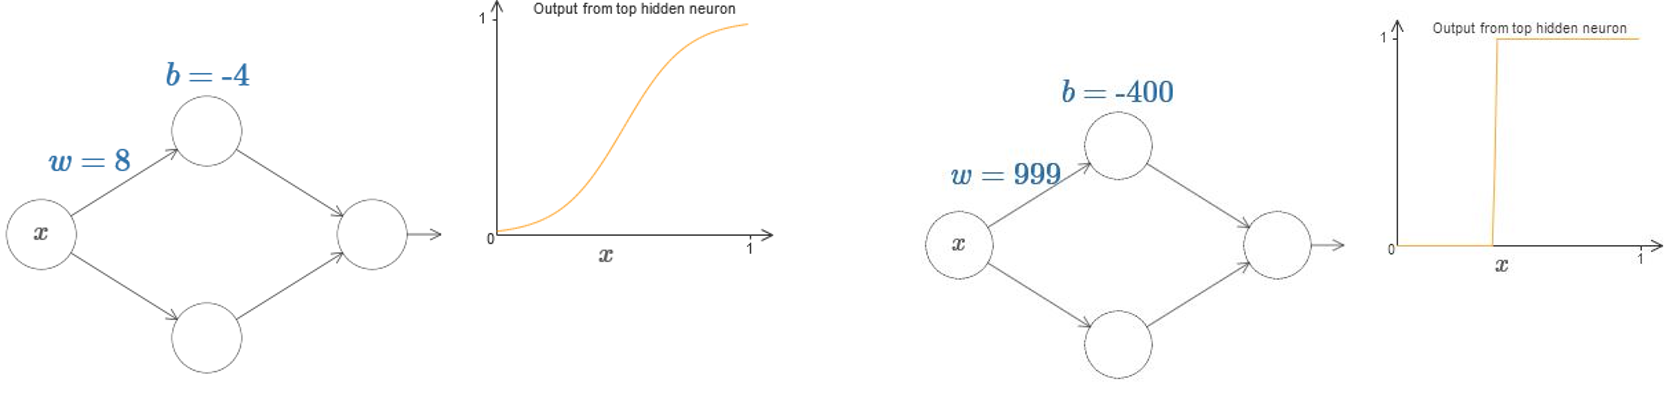
\includegraphics[width=\linewidth,keepaspectratio]{oioo}
\end{center}
{\tiny (Ref: http://neuralnetworksanddeeplearning.com/chap4.html)}
\end{frame}




%%%%%%%%%%%%%%%%%%%%%%%%%%%%%%%%%%%%%%%%%%%%%%%%%%%
\begin{frame}[fragile] \frametitle{Where step occurs?}
\begin{itemize}
\item The step is at position $s=\frac{-b}{w}$
\item Here, at $s = 0.40$
\item So, instead of $b$ and $w$, only $s$ can be used to denote a neuron.
\item It is achieved by setting $w$ to be a large value and then finding $b = -ws$
\end{itemize}
\begin{center}
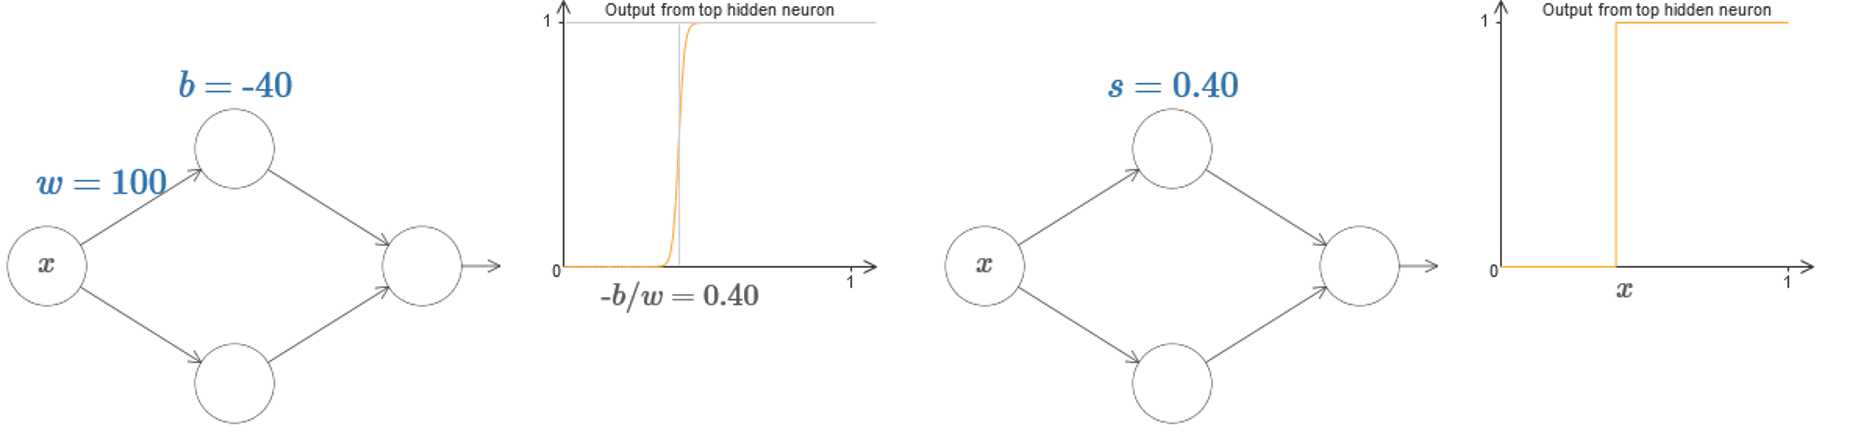
\includegraphics[width=\linewidth,keepaspectratio]{step}
\end{center}
{\tiny (Ref: http://neuralnetworksanddeeplearning.com/chap4.html)}
\end{frame}



%%%%%%%%%%%%%%%%%%%%%%%%%%%%%%%%%%%%%%%%%%%%%%%%%%%
\begin{frame}[fragile] \frametitle{Two Neurons, Two steps}
Considering both hidden neurons, the equation becomes $= g(w_1x+b_1 + w_2x+b_2)$, where $g(z) = 1/(1+ e^{-z})$
\begin{itemize}
\item Two neurons give two step functions. They decide step points.
\item These are part of hidden layer
\item Outputs from both neurons $(a1,a2)$ are as input to next neuron
\item With new weights, the output is $(w_1 a_1+w_2 a_2).$
\item Both weights control height of their respective steps


\end{itemize}
\begin{center}
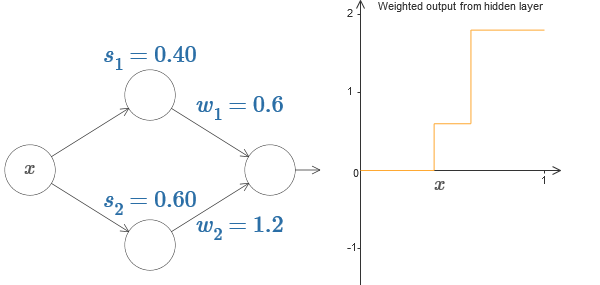
\includegraphics[width=0.65\linewidth,keepaspectratio]{twoitwos}
\end{center}
{\tiny (Ref: http://neuralnetworksanddeeplearning.com/chap4.html)}
\end{frame}

%%%%%%%%%%%%%%%%%%%%%%%%%%%%%%%%%%%%%%%%%%%%%%%%%%%
\begin{frame}[fragile] \frametitle{Universality: One input One Output}
Change in $s_1$

\begin{center}
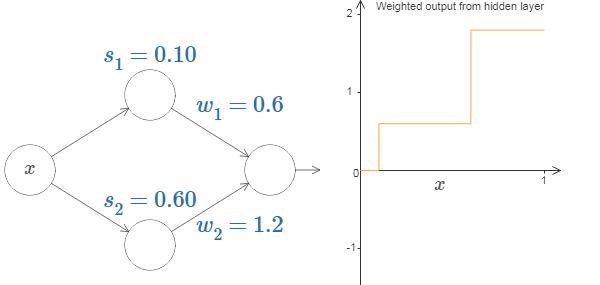
\includegraphics[width=0.5\linewidth,keepaspectratio]{dmaths12}
\end{center}
Matches at 0.60
\begin{center}
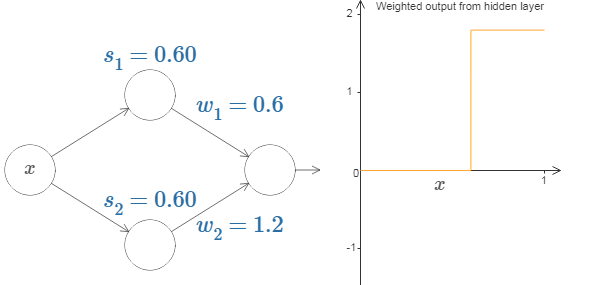
\includegraphics[width=0.5\linewidth,keepaspectratio]{dmaths13}
\end{center}

{\tiny (Ref: http://neuralnetworksanddeeplearning.com/chap4.html)}
\end{frame}

%%%%%%%%%%%%%%%%%%%%%%%%%%%%%%%%%%%%%%%%%%%%%%%%%%%
\begin{frame}[fragile] \frametitle{Universality: One input One Output}
It's particularly worth understanding what happens when $s_1$ goes past $s_2$.

Initially, bottom vertical line ($s_1$'s line) starts moving right, then the top vertical (ie $s_2$'s) starts moving to right when $s_1$ goes more than 0.60. $s_1$'s own vertical line then stays as is.
\begin{center}
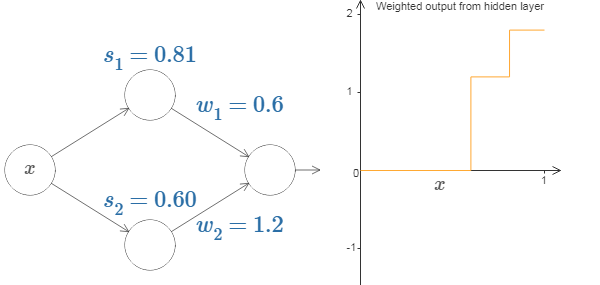
\includegraphics[width=0.5\linewidth,keepaspectratio]{dmaths14}
\end{center}

You'll see that the graph changes shape when this happens, since we have moved from a situation where the top hidden neuron is the first to be activated to a situation where the bottom hidden neuron is the first to be activated.

{\tiny (Ref: http://neuralnetworksanddeeplearning.com/chap4.html)}
\end{frame}

%%%%%%%%%%%%%%%%%%%%%%%%%%%%%%%%%%%%%%%%%%%%%%%%%%%
\begin{frame}[fragile] \frametitle{Universality: One input One Output}
Change in $s_2$

\begin{center}
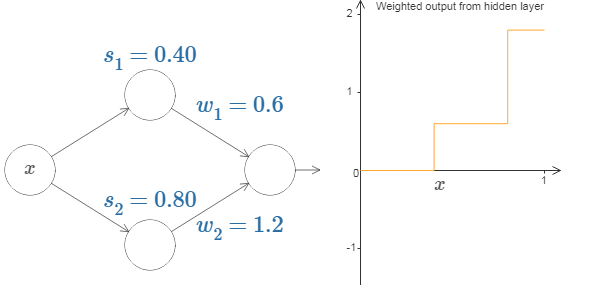
\includegraphics[width=0.5\linewidth,keepaspectratio]{dmaths15}
\end{center}
Matches at 0.40
\begin{center}
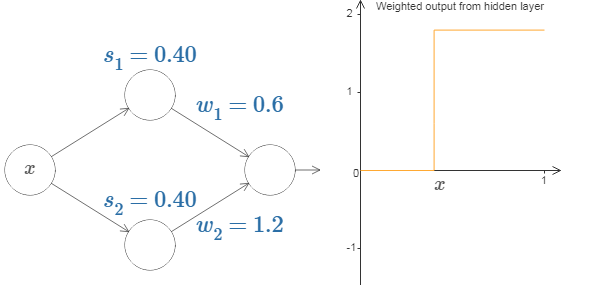
\includegraphics[width=0.5\linewidth,keepaspectratio]{dmaths16}
\end{center}

{\tiny (Ref: http://neuralnetworksanddeeplearning.com/chap4.html)}
\end{frame}

%%%%%%%%%%%%%%%%%%%%%%%%%%%%%%%%%%%%%%%%%%%%%%%%%%%
\begin{frame}[fragile] \frametitle{Universality: One input One Output}
Similar to $s_1$ its worth understanding what happens when $s_2$ goes past $s_1$.

Initially, top vertical line ($s_2$'s line) starts moving left, then the bottom vertical (ie $s_1$'s) starts moving to left when $s_2$ goes less than the common value. $s_2$'s own vertical line then stays as is.
\begin{center}
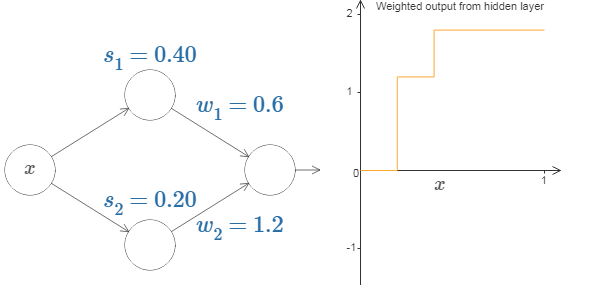
\includegraphics[width=0.5\linewidth,keepaspectratio]{dmaths17}
\end{center}

{\tiny (Ref: http://neuralnetworksanddeeplearning.com/chap4.html)}
\end{frame}

%%%%%%%%%%%%%%%%%%%%%%%%%%%%%%%%%%%%%%%%%%%%%%%%%%%
\begin{frame}[fragile] \frametitle{Universality: One input One Output}
Change in $w_1$

\begin{center}
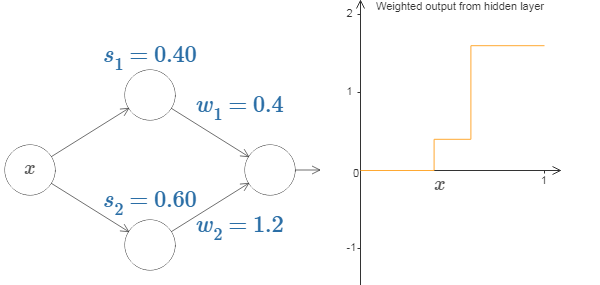
\includegraphics[width=0.5\linewidth,keepaspectratio]{dmaths18}
\end{center}

\begin{center}
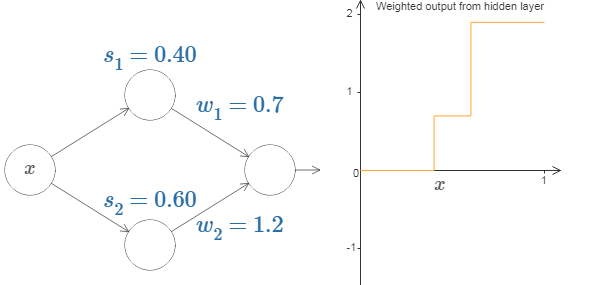
\includegraphics[width=0.5\linewidth,keepaspectratio]{dmaths19}
\end{center}

Scales the bottom step (along with it top one moves as well)

{\tiny (Ref: http://neuralnetworksanddeeplearning.com/chap4.html)}
\end{frame}

%%%%%%%%%%%%%%%%%%%%%%%%%%%%%%%%%%%%%%%%%%%%%%%%%%%
\begin{frame}[fragile] \frametitle{Universality: One input One Output}
Change in $w_2$

\begin{center}
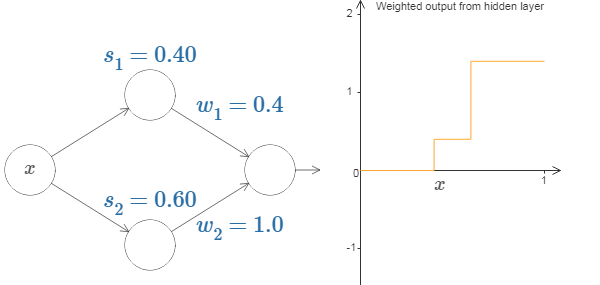
\includegraphics[width=0.5\linewidth,keepaspectratio]{dmaths20}
\end{center}

\begin{center}
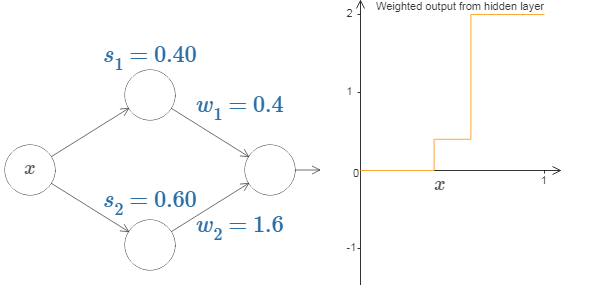
\includegraphics[width=0.5\linewidth,keepaspectratio]{dmaths21}
\end{center}

Scales the top step (along with it bottom does not move)

{\tiny (Ref: http://neuralnetworksanddeeplearning.com/chap4.html)}
\end{frame}
%%%%%%%%%%%%%%%%%%%%%%%%%%%%%%%%%%%%%%%%%%%%%%%%%%%
\begin{frame}[fragile] \frametitle{At a particular point}
\begin{itemize}
\item Setting $ w_1$ to be $0.8$ and $w_2$ to be $-0.8$. 
\item You get a ``bump'' function, which starts at point $s_1$, ends at point $s_2$, and has height $0.8$.
\item We can rescale the bump to have any height at all. Let's use a single parameter, $h$, to denote the height. To reduce clutter I'll also remove the $s_1$ and $w_1$ notations.
\item Scale it to $h = 0.6$. Making it negative, puts the bump below x axis.
\end{itemize}
\begin{center}
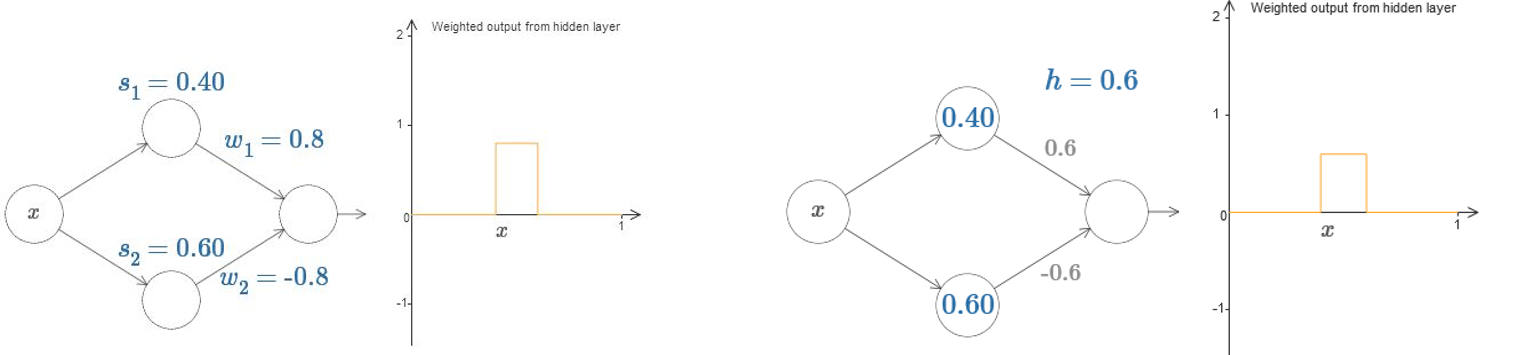
\includegraphics[width=\linewidth,keepaspectratio]{stepstep}
\end{center}
\end{frame}

%%%%%%%%%%%%%%%%%%%%%%%%%%%%%%%%%%%%%%%%%%%%%%%%%%%
\begin{frame}[fragile] \frametitle{Finally}
\begin{itemize}
\item We have a neural network which can give us a STEP.
\item We can adjust its start point by adjusting $s1$ (0.4) here
\item We can adjust its end point by adjusting $s2$ (0.6) here
\item We can adjust its height by adjusting $h$ (0.5) here
\end{itemize}
\begin{center}
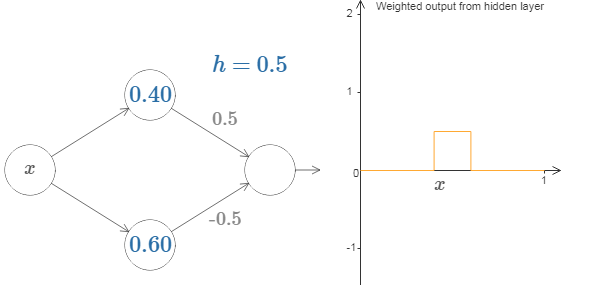
\includegraphics[width=\linewidth,keepaspectratio]{dmaths22}
\end{center}
\end{frame}


%%%%%%%%%%%%%%%%%%%%%%%%%%%%%%%%%%%%%%%%%%%%%%%%%%%
\begin{frame}[fragile] \frametitle{Want More STEPS?}

\begin{itemize}
\item Then have more pairs in the hidden layer
\item Use two sets of pairs seen earlier
\end{itemize}
\begin{center}
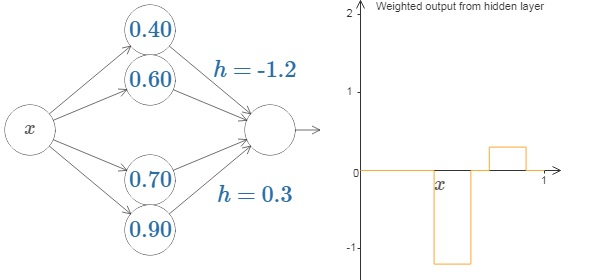
\includegraphics[width=\linewidth,keepaspectratio]{dmaths23}
\end{center}

\end{frame}

%%%%%%%%%%%%%%%%%%%%%%%%%%%%%%%%%%%%%%%%%%%%%%%%%%%
\begin{frame}[fragile] \frametitle{More in the hidden layer}
\begin{itemize}
\item Use this to get as many bumps as you want.
\item $N$ pairs of hidden neurons will give $N$ bumps of adjustable height and $x$ width.
\end{itemize}

\begin{center}
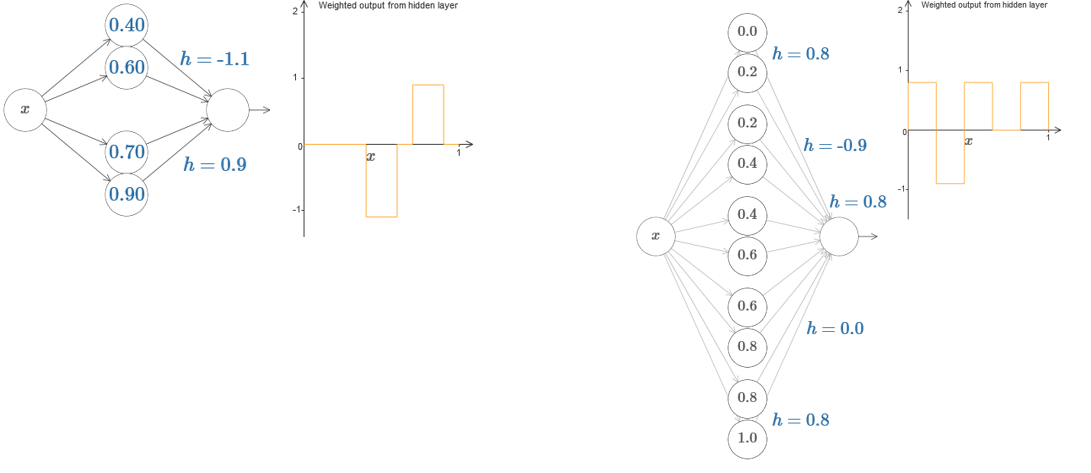
\includegraphics[width=\linewidth,keepaspectratio]{hidden}
\end{center}
{\tiny (Ref: http://neuralnetworksanddeeplearning.com/chap4.html)}
\end{frame}


%%%%%%%%%%%%%%%%%%%%%%%%%%%%%%%%%%%%%%%%%%%%%%%%%%%
\begin{frame}[fragile] \frametitle{So far}
We have crossed the hidden layer, but not the final node.
\begin{itemize}
\item We looked at combination $\sum_j w_j a_j$ output from the hidden neurons
\item Output of the network is $\sigma(\sum_j w_j a_j + b)$ where b is the bias on the output neuron. 
\item Is there some way we can achieve control over the actual output from the network?
\end{itemize}

\end{frame}

%%%%%%%%%%%%%%%%%%%%%%%%%%%%%%%%%%%%%%%%%%%%%%%%%%%
\begin{frame}[fragile] \frametitle{The Solution}
\begin{itemize}
\item We want to mimic $f(x)$
\item What we have so far is $\sigma(\sum_j w_j a_j + b)$
\item Both need to be same, ideally $\sigma(\sum_j w_j a_j + b) = f(x)$
\item Meaning, $(\sum_j w_j a_j + b) = \sigma^{-1} \circ f(x)$
\item So, for the final node/layer, instead of $\sigma$, if we had output(activation) as $\sigma^{-1} \circ f(x)$, where $\sigma^{-1}$ is just the inverse of the $\sigma$ function.
\end{itemize}

\end{frame}


%%%%%%%%%%%%%%%%%%%%%%%%%%%%%%%%%%%%%%%%%%%%%%%%%%%
\begin{frame}[fragile] \frametitle{The Solution}

That is, we want the weighted output from the hidden layer to be:
\begin{center}
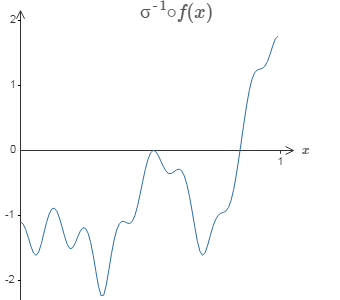
\includegraphics[width=0.5\linewidth,keepaspectratio]{dmaths24}
\end{center}

If we can use our STEPS to make this graph, then the output from the network as a whole will be a good approximation to $f(x)$ (assuming the bias on the output neuron to 0)

{\tiny (Ref: http://neuralnetworksanddeeplearning.com/chap4.html)}
\end{frame}



%%%%%%%%%%%%%%%%%%%%%%%%%%%%%%%%%%%%%%%%%%%%%%%%%%%
\begin{frame}[fragile] \frametitle{Example }
Computing a complex function
\begin{itemize}
\item $f(x)=0.2+0.4x2+0.3xsin(15x)+0.05cos(50x) = g(\sum w*a + b)$
\item We have $\sum w*a + b = g_{inv} f(x)$
\item Add hidden layer nodes, with weights and biases so that it forms a shape like shown.
\item Start with random weights and biases, add them up. See what you get. Find the diff with the goal function as error.
\end{itemize}

\end{frame}

%%%%%%%%%%%%%%%%%%%%%%%%%%%%%%%%%%%%%%%%%%%%%%%%%%%
\begin{frame}[fragile] \frametitle{The Solution}


\begin{center}
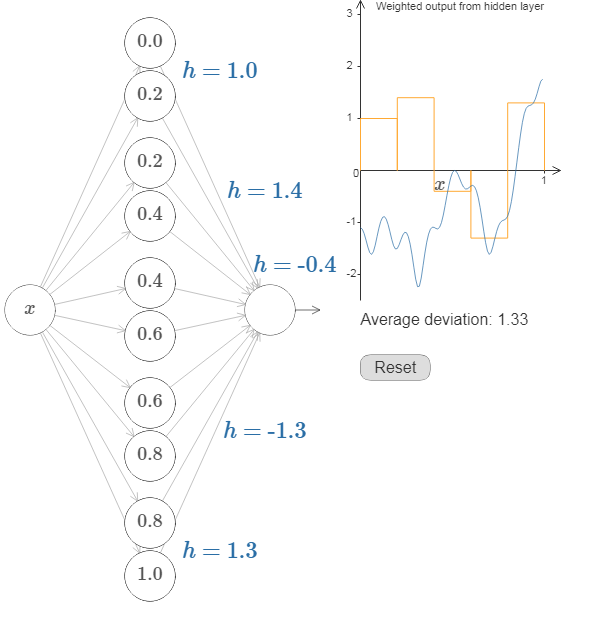
\includegraphics[width=0.6\linewidth,keepaspectratio]{dmaths25}
\end{center}

{\tiny (Ref: http://neuralnetworksanddeeplearning.com/chap4.html)}
\end{frame}


%%%%%%%%%%%%%%%%%%%%%%%%%%%%%%%%%%%%%%%%%%%%%%%%%%%
\begin{frame}[fragile] \frametitle{Example }
Computing a complex function
\begin{itemize}
\item So far the fitting to graph is not good. 
\item There is a lot of deviation/error.
\item We could easily do much better, merely by increasing the number of pairs of hidden neurons, allowing more bumps.
\item We can adjust weights and biases at each arrows, nodes to get needed STEPS.
\end{itemize}

\end{frame}


%%%%%%%%%%%%%%%%%%%%%%%%%%%%%%%%%%%%%%%%%%%%%%%%%%%
\begin{frame}[fragile] \frametitle{Back-propagation}
\begin{itemize}
\item Trying to approximate $y = f(x)$
\item Model predicts $y' = g(x, \theta)$, where g is some model function and it depends on input $x$ (obviously) and some extra parameters $\theta$ (say, weights \& biases), collectively called $\theta$
\item $Error = Loss = J(y,y')$ is thus $J (\theta)$
\item Idea is to minimize `J' wrt $\theta$ ie wrt Weights $W$ and biases $b$
\item Derivatives gives slope and thus direction where $J$ is reducing
\item $\theta_{new} = \theta_{old} - \alpha \frac{\partial J}{\partial \theta}$
\item Local minima
\end{itemize}
\end{frame}

%%%%%%%%%%%%%%%%%%%%%%%%%%%%%%%%%%%%%%%%%%%%%%%%%%%
\begin{frame}[fragile] \frametitle{Back-propagation}
\begin{center}
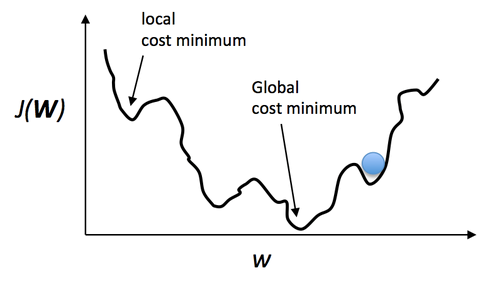
\includegraphics[width=0.6\linewidth,keepaspectratio]{backprop}
\end{center}
{\tiny (Ref: http://neuralnetworksanddeeplearning.com/chap4.html)}
\end{frame}


%%%%%%%%%%%%%%%%%%%%%%%%%%%%%%%%%%%%%%%%%%%%%%%%%%%
\begin{frame}[fragile] \frametitle{Back-propagation}
\begin{itemize}
\item Adjust $w$ and $b$ in iterations
\item Till it matches the curve
\item Back-propagation is automatic way of calculating $w$ and $b$
\item Gradient descent algorithm
\end{itemize}
\end{frame}

%%%%%%%%%%%%%%%%%%%%%%%%%%%%%%%%%%%%%%%%%%%%%%%%%%%
\begin{frame}[fragile] \frametitle{Back-propagation}
\begin{center}
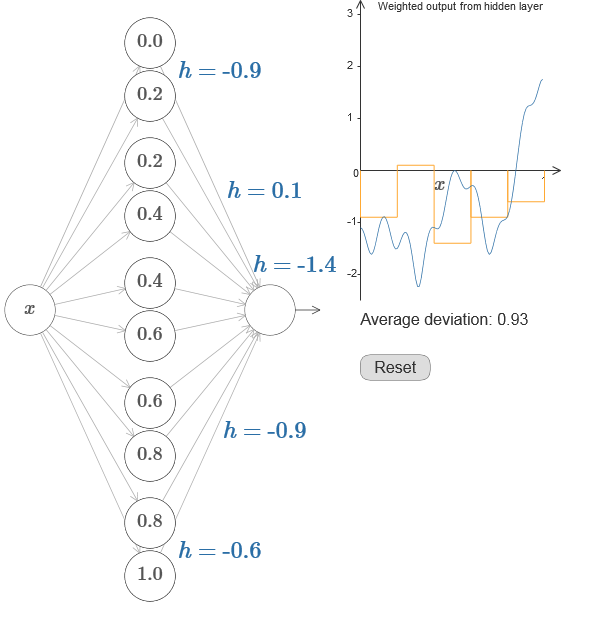
\includegraphics[width=0.6\linewidth,keepaspectratio]{backprop2}
\end{center}
{\tiny (Ref: http://neuralnetworksanddeeplearning.com/chap4.html)}
\end{frame}



%%%%%%%%%%%%%%%%%%%%%%%%%%%%%%%%%%%%%%%%%%%%%%%%%%%
\begin{frame}[fragile] \frametitle{Many input variables}
With inputs $x$ and $y$ the output is no longer single dimensional curve but a 2 dimensional surface.

\begin{center}
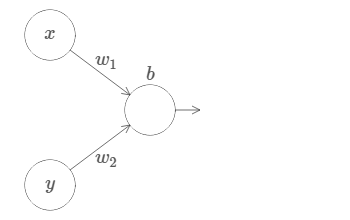
\includegraphics[width=0.6\linewidth,keepaspectratio]{dmaths26}
\end{center}
{\tiny (Ref: http://neuralnetworksanddeeplearning.com/chap4.html)}

\end{frame}

%%%%%%%%%%%%%%%%%%%%%%%%%%%%%%%%%%%%%%%%%%%%%%%%%%%
\begin{frame}[fragile] \frametitle{Many input variables}

\begin{itemize}
\item With w2=0 the input y makes no difference to the output from the neuron. It's as though x is the only input.
\item $w_2=0$ the input $y$ makes no difference to the output from the neuron. It's as though $x$ is the only input.
\item If $w_1$ is made very high, it becomes a step function in $x$
\item $s_x = -b/w_1$
\end{itemize}

\begin{center}
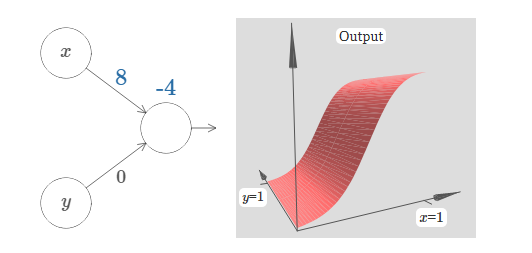
\includegraphics[width=0.6\linewidth,keepaspectratio]{dmaths27}
\end{center}
{\tiny (Ref: http://neuralnetworksanddeeplearning.com/chap4.html)}
\end{frame}

%%%%%%%%%%%%%%%%%%%%%%%%%%%%%%%%%%%%%%%%%%%%%%%%%%%
\begin{frame}[fragile] \frametitle{Many input variables}
Let's redo the above using the position of the step as the parameter:

\begin{center}
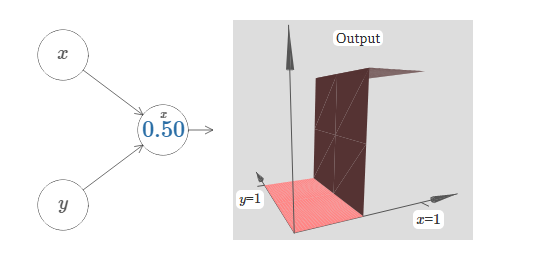
\includegraphics[width=0.6\linewidth,keepaspectratio]{dmaths28}
\end{center}


\begin{itemize}
\item Wsed $w_1=1000$ (large) and the weight $w_2=0$. 
\item The number on the neuron (0.5) is the step point, and the little $x$ above the number reminds us that the step is in the $x$ direction.
\end{itemize}


{\tiny (Ref: http://neuralnetworksanddeeplearning.com/chap4.html)}
\end{frame}


%%%%%%%%%%%%%%%%%%%%%%%%%%%%%%%%%%%%%%%%%%%%%%%%%%%
\begin{frame}[fragile] \frametitle{Many input variables}
Similarly it's also possible to get a step function in the y direction, by making the weight on the y input very large (say, $w_2=1000$), and the weight on the x equal to 0, i.e., $w_1=0$:

\begin{center}
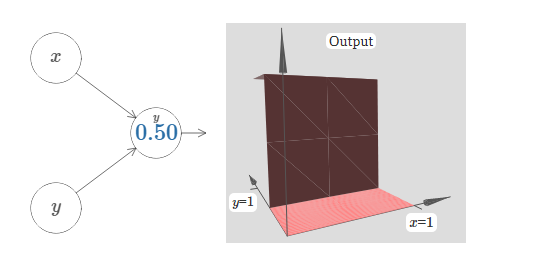
\includegraphics[width=0.6\linewidth,keepaspectratio]{dmaths29}
\end{center}


The number on the neuron is again the step point, and in this case the little y above the number reminds us that the step is in the y direction. 

{\tiny (Ref: http://neuralnetworksanddeeplearning.com/chap4.html)}
\end{frame}


%%%%%%%%%%%%%%%%%%%%%%%%%%%%%%%%%%%%%%%%%%%%%%%%%%%
\begin{frame}[fragile] \frametitle{Many input variables}

\begin{itemize}
\item We can use the step functions we've just constructed to compute a three-dimensional bump function.
\item  To do this, we use two neurons, each computing a step function in the x direction. 
\item Then we combine those step functions with weight h and -h, respectively, where h is the desired height of the bump.
\end{itemize}

\begin{center}
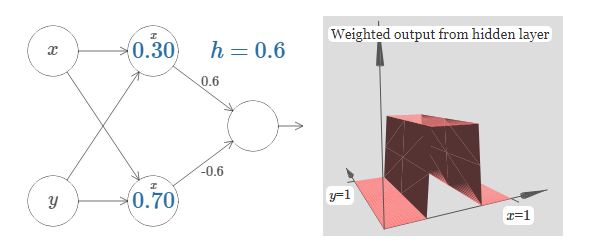
\includegraphics[width=0.6\linewidth,keepaspectratio]{dmaths30}
\end{center}
{\tiny (Ref: http://neuralnetworksanddeeplearning.com/chap4.html)}
\end{frame}

%%%%%%%%%%%%%%%%%%%%%%%%%%%%%%%%%%%%%%%%%%%%%%%%%%%
\begin{frame}[fragile] \frametitle{Surface Step}
\begin{itemize}
\item Use two neurons, each computing a step function in the $x$ direction. 
\item Combine those step functions with weight $h$ and $-h$, the desired height of the bump.
\item $0.3$ is first step interval on $x$ and $0.7$ is second. Height is $h$
\item Same can be in $y$
\end{itemize}

\end{frame}

%%%%%%%%%%%%%%%%%%%%%%%%%%%%%%%%%%%%%%%%%%%%%%%%%%%
\begin{frame}[fragile] \frametitle{Surface Step}
\begin{center}
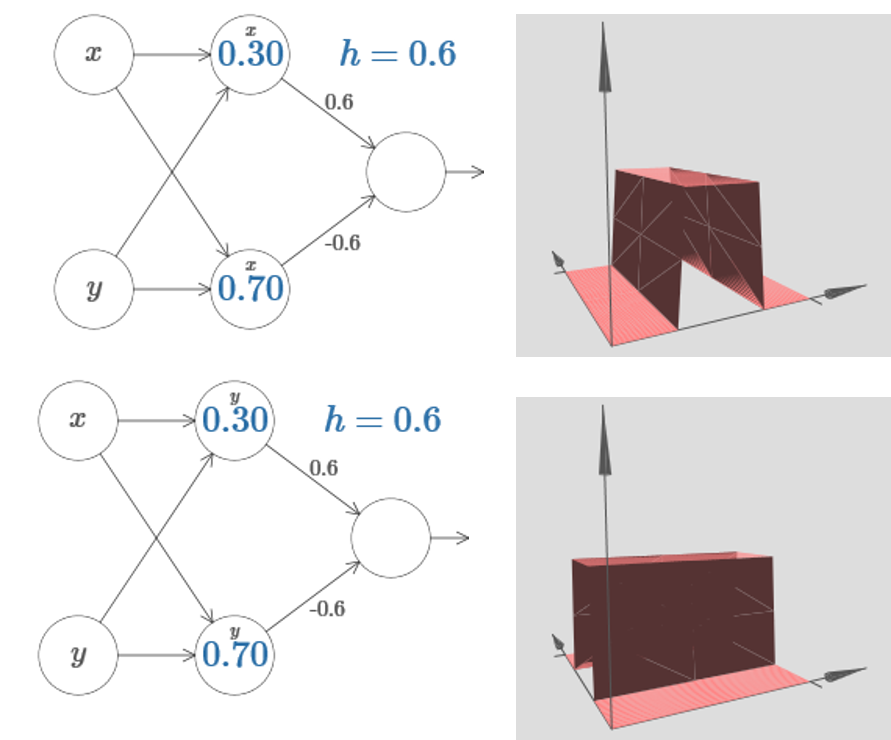
\includegraphics[width=0.7\linewidth,keepaspectratio]{surfstep}
\end{center}
{\tiny (Ref: http://neuralnetworksanddeeplearning.com/chap4.html)}
\end{frame}



%%%%%%%%%%%%%%%%%%%%%%%%%%%%%%%%%%%%%%%%%%%%%%%%%%%
\begin{frame}[fragile] \frametitle{Combine $x$ and $y$ steps}
\begin{itemize}
\item Add up two bump functions, one in the $x$ direction, the other in the $y$ direction, both of height $h$
\item The addition is a Tower like function
\item We can use such many towers to approximate any surface(2D) function
\item To make output Boolean, we use threshold, above $1$, below $0$.
\end{itemize}
\end{frame}


%%%%%%%%%%%%%%%%%%%%%%%%%%%%%%%%%%%%%%%%%%%%%%%%%%%
\begin{frame}[fragile] \frametitle{Combine $x$ and $y$ steps}
\begin{center}
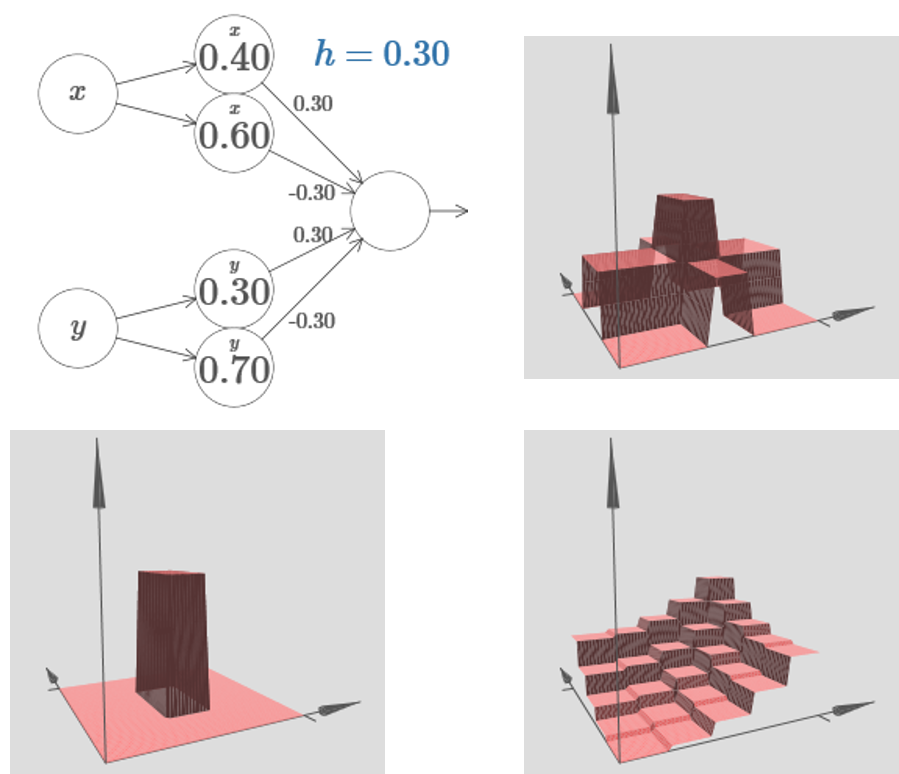
\includegraphics[width=0.7\linewidth,keepaspectratio]{combxy}
\end{center}
{\tiny (Ref: http://neuralnetworksanddeeplearning.com/chap4.html)}
\end{frame}



%%%%%%%%%%%%%%%%%%%%%%%%%%%%%%%%%%%%%%%%%%%%%%%%%%%
\begin{frame}[fragile] \frametitle{More variables}
What about functions of more than two variables?
\begin{itemize}
\item With three variables$ x_1,x_2,x_3$ the following network can be used to compute a function in four dimensions
\item $x_1$ is between $s_1$ and $t_1$; $x_2$ is between $s_2$ and $t_2$; and $x_3$ is between $s_3$ and $t_3$. The network is 0 everywhere else. 
\end{itemize}

\begin{center}
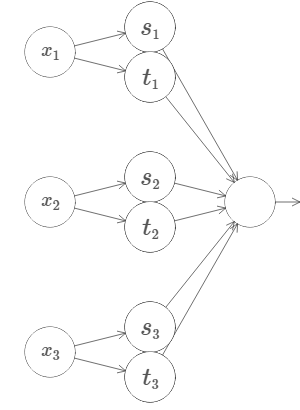
\includegraphics[width=0.3\linewidth,keepaspectratio]{dmaths31}
\end{center}
{\tiny (Ref: http://neuralnetworksanddeeplearning.com/chap4.html)}
\end{frame}

%%%%%%%%%%%%%%%%%%%%%%%%%%%%%%%%%%%%%%%%%%%%%%%%%%%
\begin{frame}[fragile] \frametitle{Next}
What about functions of more than two variables?
\begin{itemize}
\item Multiple output function ie  $f(x_1, \ldots, x_m) \in R^n$ can be regarded as $n$ separate real-valued functions
\item $f^1(x_1,\ldots, x_m), f^2(x_1, \ldots, x_m)$ and so on.
\item So we create a network approximating $f_1$, another network for $f_2$, and so on. 
\item And then we simply glue all the networks together. 
\end{itemize}


{\tiny (Ref: http://neuralnetworksanddeeplearning.com/chap4.html)}
\end{frame}

%%%%%%%%%%%%%%%%%%%%%%%%%%%%%%%%%%%%%%%%%%%%%%%%%%%
\begin{frame}[fragile] \frametitle{Conclusion}
\begin{itemize}
\item ANY continuous function can be modeled using Neural Network, albeit approximately, with just one hidden layer.
\item  Then, why we would ever be interested in deep networks, i.e., networks with many hidden layers?
\item Deep networks have a hierarchical structure which makes them particularly well adapted to learn the hierarchies of knowledge that seem to be useful in solving real-world problems, such as in Image Recognition. 
\end{itemize}


{\tiny (Ref: http://neuralnetworksanddeeplearning.com/chap4.html)}
\end{frame}

% %%%%%%%%%%%%%%%%%%%%%%%%%%%%%%%%%%%%%%%%%%%%%%%%%%%%%%%%%%%
% \begin{frame}[fragile]\frametitle{End - The Truth}
% \begin{center}
% 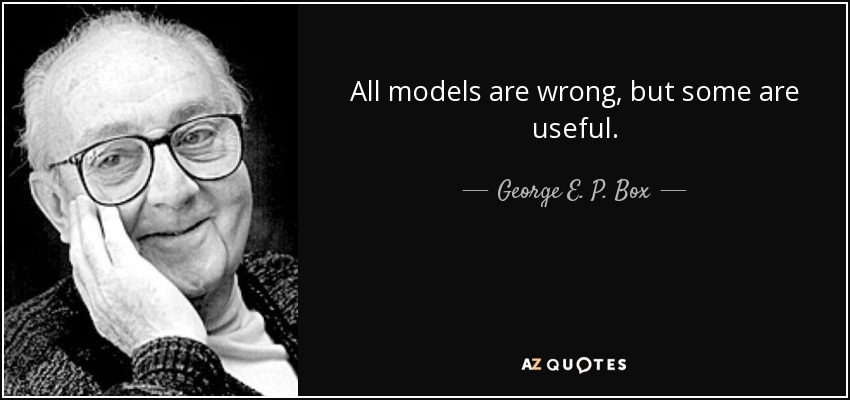
\includegraphics[width=\linewidth,keepaspectratio]{boxquote}
% \end{center}
% \end{frame}
